\documentclass[a4paper,12pt]{extarticle}
\usepackage{geometry}
\usepackage[T1]{fontenc}
\usepackage[utf8]{inputenc}
\usepackage[english,russian]{babel}
\usepackage{amsmath}
\usepackage{amsthm}
\usepackage{amssymb}
\usepackage{fancyhdr}
\usepackage{setspace}
\usepackage{graphicx}
\usepackage{colortbl}
\usepackage{tikz}
\usepackage{pgf}
\usepackage{subcaption}
\usepackage{listings}
\usepackage{indentfirst}
\usepackage{comment}
\usepackage[
backend=biber,
style=numeric,
maxbibnames=99
]{biblatex}
% \addbibresource{refs.bib}
% \usepackage[backend=biber,style=numeric,sorting=none]{biblatex}
\addbibresource{refs.bib}

\usepackage[hidelinks]{hyperref}




\usepackage[colorlinks,citecolor=blue,linkcolor=blue,bookmarks=false,hypertexnames=true, urlcolor=blue]{hyperref} 
\usepackage{indentfirst}
\usepackage{mathtools}
\usepackage{booktabs}
\usepackage[flushleft]{threeparttable}
\usepackage{tablefootnote}

\usepackage{chngcntr} % нумерация графиков и таблиц по секциям
\counterwithin{table}{section}
\counterwithin{figure}{section}

\graphicspath{{graphics/}}%путь к рисункам

\makeatletter
% \renewcommand{\@biblabel}[1]{#1.} % Заменяем библиографию с квадратных скобок на точку:
\makeatother

\geometry{left=2.5cm}% левое поле
\geometry{right=1.0cm}% правое поле
\geometry{top=2.0cm}% верхнее поле
\geometry{bottom=2.0cm}% нижнее поле
\setlength{\parindent}{1.25cm}
\renewcommand{\baselinestretch}{1.5} % междустрочный интервал


\newcommand{\bibref}[3]{\hyperlink{#1}{#2 (#3)}} % biblabel, authors, year
\addto\captionsrussian{\def\refname{Список литературы (или источников)}} 

\renewcommand{\theenumi}{\arabic{enumi}}% Меняем везде перечисления на цифра.цифра
\renewcommand{\labelenumi}{\arabic{enumi}}% Меняем везде перечисления на цифра.цифра
\renewcommand{\theenumii}{.\arabic{enumii}}% Меняем везде перечисления на цифра.цифра
\renewcommand{\labelenumii}{\arabic{enumi}.\arabic{enumii}.}% Меняем везде перечисления на цифра.цифра
\renewcommand{\theenumiii}{.\arabic{enumiii}}% Меняем везде перечисления на цифра.цифра
\renewcommand{\labelenumiii}{\arabic{enumi}.\arabic{enumii}.\arabic{enumiii}.}% Меняем везде перечисления на цифра.цифра

\begin{document}
\begin{titlepage}
\newpage

{\setstretch{1.0}
\begin{center}
ПРАВИТЕЛЬСТВО РОССИЙСКОЙ ФЕДЕРАЦИИ\\
ФГАОУ ВО НАЦИОНАЛЬНЫЙ ИССЛЕДОВАТЕЛЬСКИЙ УНИВЕРСИТЕТ\\
«ВЫСШАЯ ШКОЛА ЭКОНОМИКИ»
\\
\bigskip
Факультет компьютерных наук\\
Образовательная программа «Прикладная математика и информатика»
\end{center}
}

\vspace{2em}
УДК 004.8 % Для программного проекта эту строку можно убрать.
\vspace{4em}

\begin{center}
% Выберите нужный тип проекта.
{\bf Отчет об исследовательском проекте на тему:}\\
%{\bf Отчет о командном исследовательском проекте на тему:}\\
%{\bf Отчет о программном проекте на тему:}\\
%{\bf Отчет о командном программном проекте на тему:}\\
{\bf Факторы воспроизведения скрытых данных в мультимодальных моделях документов}\\
% Эта строка нужна только для промежуточной сдачи плана.
(промежуточный, этап 1)
\end{center}

\vspace{2em}

{\bf Выполнил студент: \vspace{2mm}}
%{\bf Выполнили студенты: \vspace{2mm}}

{\setstretch{1.1}
\begin{tabular}{l@{\hskip 1.5cm}l}
группы \#БПМИ234, 3 курса & Крамин Карим Тимурович \\
%группы \#БПМИ172, 3 курса & Петров Андрей Алексеевич \\
%группы \#БПМИ173, 3 курса & Иванов Андрей Алексеевич 
\end{tabular}}

% Обычно достаточно одного руководителя. Если есть соруководитель или консультант, их можно добавить ниже.

% Официальный руководитель из ВШЭ.
\vspace{1em}
{\bf Принял руководитель проекта: \vspace{2mm}}

{\setstretch{1.1}
\begin{tabular}{l}
Бурлова Альбина Сергеевна\\
Научный сотрудник\\
Факультет компьютерных наук НИУ ВШЭ 
\end{tabular}}

% Соруководитель, если он есть.
%\vspace{1em}
%{\bf Соруководитель: \vspace{2mm}}%это ваш официальный научник

%{\setstretch{1.1}
%\begin{tabular}{l}
%Петрова Надежда Александровна\\
%Инженер-исследователь\\
%ОАО Компания "Нейросети и деревья" 
%\end{tabular}}

% Консультант, если он есть.
%\vspace{1em}
%{\bf Консультант: \vspace{2mm}}%это ваш официальный научник

%{\setstretch{1.1}
%\begin{tabular}{l}
%Иванова Надежда Александровна\\
%Инженер-исследователь\\
%ОАО Компания "Нейросети и деревья" 
%\end{tabular}}

\vspace{\fill}

\begin{center}
Москва 2026
\end{center}

\end{titlepage}
% это титульный лист - выберите подходящий вам из имеющихся в проекте вариантов (kr - курсовая работа у 3 курса, vkr - выпускная квалификационная работа у 4 курса)
\newpage
\setcounter{page}{2}

{
	\hypersetup{linkcolor=black}
	\tableofcontents
}

\newpage

\newpage
\section*{Аннотация}   % this is how to use russian
Проект исследует способность современных мультимодальных моделей анализа документов воспроизводить скрытые или замаскированные поля после обезличивания входных данных, а также факторы, влияющие на возникновение данного эффекта. Основной акцент делается на анализе вклада визуального канала изображения документа и текстового канала распознанного текста, а также на изменении риска восстановления информации при различных процедурах маскирования, удаления данных и ограничения доступного контекста. Эксперименты предполагается проводить в задачах вопрос-ответ по документам и близких приватностных постановках, направленных на выявление утечек информации через одну или обе модальности, включая случаи воспроизведения данных при отсутствии прямых релевантных фрагментов входа.

\addcontentsline{toc}{section}{Аннотация}

\section*{Ключевые слова}
Мультимодальные модели документов,
анализ документов,
анонимизация данных,
воспроизведение скрытой информации, DocVQA, визуально-языковые модели, приватность машинного обучения, обезличивание входных данных
\pagebreak

\section{Введение}

\subsection{Описание предметной области}

В последние годы методы машинного обучения широко применяются для автоматизации анализа документов, включая задачи извлечения информации, классификации и вопрос-ответ по документам. Современные мультимодальные модели позволяют обрабатывать не только текст, полученный с помощью оптического распознавания символов (OCR), но и изображение документа, а также учитывать пространственную структуру элементов на странице. Такие подходы демонстрируют высокое качество на стандартных наборах данных и активно используются в банковских, юридических и государственных информационных системах.

При этом многие документы содержат чувствительную информацию, включая персональные данные, финансовые сведения и различные идентификаторы. Для защиты приватности на практике применяются процедуры обезличивания входных данных, предполагающие маскирование или удаление соответствующих полей в изображении документа и распознанном тексте. Предполагается, что после таких преобразований модели не имеют доступа к скрытым данным и не способны воспроизводить их в процессе анализа.

Однако ряд исследований показывает, что нейросетевые модели могут частично восстанавливать удалённую информацию, используя контекст и статистические закономерности данных. Это ставит под сомнение надёжность стандартных подходов к анонимизации и требует более детального изучения рисков утечек информации в системах анализа документов.

\subsection{Постановка задачи}

Большинство существующих работ, посвящённых проблемам приватности в машинном обучении, фокусируется преимущественно на текстовых языковых моделях и значительно реже рассматривает мультимодальные модели анализа документов. В частности, недостаточно изучен вклад визуального представления документа и OCR-текста в воспроизведение скрытых данных после процедур обезличивания. Также отсутствует систематический анализ влияния различных способов маскирования и ограничения контекста на риск восстановления конфиденциальной информации.

В рамках данной работы ставится задача исследовать факторы, влияющие на воспроизведение скрытых и потенциально конфиденциальных данных в мультимодальных моделях анализа документов после обезличивания входных данных. Особое внимание уделяется оценке вклада визуального и текстового каналов, а также устойчивости различных процедур анонимизации.

Для решения поставленной задачи планируется использовать постановку вопрос-ответ по документам на основе набора данных DocVQA. В экспериментах будут применяться процедуры обезличивания как к изображению документа, так и к распознанному тексту, включая маскирование чувствительных областей, удаление отдельных фрагментов и ограничение доступного контекста. В качестве моделей предполагается рассмотреть современные мультимодальные архитектуры, работающие с визуальной и текстовой информацией.

\subsection{Структура работы}

Дальнейшая структура работы организована следующим образом. Во втором разделе представлен обзор существующих исследований в области мультимодального анализа документов и проблем приватности нейросетевых моделей. В третьем разделе описывается экспериментальная постановка, используемые модели и процедуры обезличивания входных данных. Затем приводятся результаты экспериментов и их анализ. В заключении формулируются основные выводы и обсуждаются возможные направления дальнейших исследований.





\section{Обзор литературы}

\subsection{Мультимодальные модели для анализа документов}

Анализ документов отличается от классической обработки текста тем, что информация в них представлена не только в виде текста, но и в визуальной форме и пространственной структуре страницы. Существенную роль играют шрифты, таблицы, расположение блоков и форматирование. В связи с этим были разработаны мультимодальные модели Document AI, объединяющие изображение документа, OCR-текст и layout-информацию в едином представлении.

Широкое распространение получили трансформерные архитектуры, учитывающие пространственную структуру документа и совместно моделирующие текстовые и визуальные признаки. Одной из таких моделей является LayoutLMv3, использующая единый механизм предобучения для текстовых и визуальных компонентов и демонстрирующая высокое качество на задачах документного анализа, включая DocVQA \cite{layoutlmv3} .

Другой подход основан на отказе от внешнего OCR и обработке документа напрямую как изображения. Модель Donut обучается end-to-end для генерации текстовых ответов по изображению документа и не требует отдельного этапа распознавания текста \cite{donut}. Это позволяет избежать ошибок OCR, но делает модель полностью зависимой от визуального канала.

В контексте данного исследования важно, что модели типа LayoutLMv3 используют как изображение, так и OCR-текст, тогда как Donut опирается только на визуальное представление документа. Это позволяет рассматривать вклад каждой модальности отдельно при анализе воспроизведения скрытых данных.

\subsection{Постановка DocVQA и извлечение чувствительных полей}

Задача Document Visual Question Answering (DocVQA) заключается в получении ответа на текстовый вопрос по изображению документа, иногда с использованием OCR-текста \cite{docvqa}. В отличие от классических задач визуального вопрос-ответа, ответы в DocVQA часто соответствуют конкретным значениям полей документа, таким как имена, даты, суммы и идентификаторы.

Это делает DocVQA удобной экспериментальной постановкой для изучения приватности, поскольку многие ответы представляют собой потенциально конфиденциальную информацию. В условиях обезличивания естественным является сценарий, при котором чувствительные поля скрываются на входе, но модель тем не менее пытается восстановить исходные значения.

\subsection{Приватность моделей}

Воспроизведение скрытых данных связано с более широкой проблемой приватности нейросетевых моделей. Для крупных языковых моделей показано, что при определённых запросах возможно извлечение фрагментов обучающих данных, включая редкие и чувствительные последовательности \cite{carlini_extraction}. Обзорные работы подчёркивают, что подобные утечки являются системным риском и зависят как от свойств данных, так и от протокола взаимодействия с моделью \cite{tde_survey_2023}.

Существуют также атаки типа model inversion, направленные на восстановление информации об обучающих данных по выходам модели \cite{zhang_mi_cvpr20}. Недавние исследования показывают, что аналогичные угрозы сохраняются и для vision-language моделей, включая атаки membership inference, позволяющие определять принадлежность примеров к данным обучения \cite{vlm_mia_neurips24}. Это указывает на необходимость отдельного анализа приватности для мультимодальных систем.

\subsection{Анонимизация документов и устойчивость моделей}

На практике обезличивание документов обычно реализуется как предобработка входных данных. К распространённым методам относятся маскирование чувствительных областей изображения, удаление или замена соответствующих токенов в OCR-тексте, а также ограничение доступного контекста документа.

Интуитивно предполагается, что после таких преобразований модель не сможет воспроизводить скрытую информацию. Однако для документных моделей важную роль играют косвенные признаки, включая структуру шаблонов, окружение полей и статистические зависимости. Кроме того, исследования устойчивости layout-моделей показывают, что изменение структуры документа может существенно влиять на поведение моделей \cite{layoutlm_robust_acl23}. Это означает, что даже после удаления явных фрагментов могут сохраняться сигналы, достаточные для частичного восстановления скрытых данных.

В условиях мультимодальности возможны и более сложные сценарии, при которых утечка происходит через один канал при корректном обезличивании другого либо за счёт их комбинации. Систематический анализ таких эффектов для задач анализа документов в литературе пока представлен ограниченно.

\subsection{Позиционирование данного исследования}

Существующие работы охватывают отдельные аспекты рассматриваемой проблемы: развитие мультимодальных моделей для анализа документов и DocVQA \cite{layoutlmv3,donut,docvqa}, исследования утечек и атак на приватность нейросетевых моделей \cite{carlini_extraction,tde_survey_2023,zhang_mi_cvpr20} и анализ рисков для vision-language архитектур \cite{vlm_mia_neurips24}. 

Вместе с тем остаётся недостаточно изученным сценарий воспроизведения скрытых полей после обезличивания входных данных в задачах анализа документов с явным разделением вкладов визуального и текстового каналов.

Данное исследование направлено на восполнение этого пробела за счёт проведения систематических экспериментов, в которых процедуры анонимизации и ограничения контекста рассматриваются как факторы анализа, а модели запускаются в режимах с доступом только к изображению, только к OCR-тексту и к обеим модальностям. Такой подход позволяет количественно оценить риск восстановления скрытых данных и выявить уязвимые сценарии обезличивания.



\section{Постановка задачи и методология}
\label{sec:methodology}

\subsection{Формальная постановка задачи}
\label{sec:problem_statement}

Мы рассматриваем генеративную модель~$\mathcal{M}$, которая по изображению документа~$x$ и текстовому вопросу~$q$ порождает ответ~$\hat{a} = \mathcal{M}(x, q)$. Ответ, как правило, соответствует значению конкретного поля документа: дате, денежной сумме, имени, идентификатору. Модель дообучается на выборке~$\mathcal{D}_{\mathrm{train}} = \{(x_i, q_i, a_i)\}_{i=1}^{N}$, после чего мы проверяем, возникает ли утечка информации о данных обучения.

Мы анализируем два типа утечки.

Первый~--- membership inference attack (MIA). По выходам модели~$\mathcal{M}$ на примере~$(x, q, a)$ мы определяем, входил ли он в~$\mathcal{D}_{\mathrm{train}}$. Формально это задача бинарной классификации: класс~$1$~--- пример из обучающей выборки (seen), класс~$0$~--- пример, которого модель не видела при обучении (unseen). В качестве скоринговых функций мы используем cross-entropy loss и среднюю log-вероятность сгенерированных токенов. Качество атаки оценивается по AUC-ROC: значение~$0{,}5$ означает, что модель не различает seen и unseen; значение, близкое к~$1{,}0$,~--- что membership leakage выражено.

Второй~--- data extraction attack. Мы проверяем, способна ли дообученная модель восстановить значение поля, которое было скрыто на входном изображении или удалено из OCR-текста. Модель получает отредактированное изображение~$\tilde{x}$ (целевое поле замаскировано) и вопрос~$q$, а предсказание~$\hat{a} = \mathcal{M}(\tilde{x}, q)$ сравнивается с эталонным ответом~$a$. Если модель точно воспроизводит скрытое значение на seen-примерах, но не на unseen~--- это сигнал memorization.

\subsection{Данные}
\label{sec:data}

В качестве основы мы используем датасет \texttt{pixparse/docvqa-single-page-questions}~\cite{docvqa}~--- набор пар <<изображение документа + вопрос>> с текстовым ответом. Документы в датасете~--- формы, письма, инвойсы, отчёты~--- содержат поля разной природы: даты, суммы, имена, идентификаторы, адреса.

Для анализа утечек по типам полей мы разметили каждую пару~$(q, a)$ гибридным пайплайном: сначала детерминированные правила (принимаются при confidence~$\geq 0{,}93$), затем, если правило не сработало, языковая модель GigaChat. Качество пайплайна мы проверили на~300 вручную размеченных примерах: overall accuracy~$= 0{,}84$; правила дали accuracy~$= 0{,}88$ (на~132 примерах), LLM~--- accuracy~$= 0{,}80$ (на~168 примерах).

Результирующие fine-grained типы мы свернули в шесть укрупнённых категорий (coarse field types):
\begin{itemize}
    \item DATE~--- даты и временные метки (из DATE\_TIME);
    \item AMOUNT~--- денежные суммы, количества, проценты (из MONEY, QUANTITY, PERCENTAGE);
    \item ID~--- идентификаторы и ссылки на документы (из IDENTIFIER, DOCUMENT\_REFERENCE);
    \item PERSON~--- имена людей (из PERSON\_NAME);
    \item ORG~--- названия организаций (из ORG\_NAME);
    \item CONTACT\_ADR~--- адреса и контактные данные (из ADDRESS, CONTACT).
\end{itemize}

Укрупнение нужно, чтобы в каждой подгруппе было достаточно примеров для осмысленного анализа и чтобы строить стратифицированные выборки с равным представительством каждого типа.

Для экспериментов мы формируем два множества по~200 примеров каждое: seen (стратифицированная подвыборка из train split) и unseen (стратифицированная подвыборка из validation split). При~200 примерах и~6 типах каждый тип получает 33--34 примера. Для каждого примера в benchmark сохраняются: изображение документа, OCR-токены, bounding box ответа, вопрос, эталонный ответ и метаданные типа поля.

\subsection{Модели}
\label{sec:models}

Мы сравниваем три мультимодальные генеративные модели разного масштаба.

Florence-2-base~\cite{florence2}~--- encoder-decoder модель от Microsoft с~${\sim}230$M параметров. Работает только с изображением: на входе~--- изображение документа и текстовый промпт, на выходе~--- строковый ответ. Компактный размер позволяет дообучать все параметры.

Qwen2-VL-2B-Instruct~\cite{qwen2vl}~--- мультимодальная модель из семейства Qwen с~${\sim}2$B параметров. Принимает изображение и текстовый промпт в формате диалога. Мы используем два режима: image-only (только изображение) и image+OCR (OCR-текст добавляется в промпт).

Qwen2-VL-7B-Instruct~\cite{qwen2vl}~--- та же архитектура, но~${\sim}7$B параметров. Используется в режиме image-only.

Модели выбраны так, чтобы покрыть диапазон от сотен миллионов до миллиардов параметров и сопоставить encoder-decoder архитектуру (Florence) с decoder-only (Qwen). Различие масштабов и архитектур позволяет проверить, как эти факторы влияют на privacy leakage.

\subsection{Процедура дообучения}
\label{sec:finetuning}

Мы проводим эксперименты в двух режимах.

Режим~v1 (practical setup): каждая модель дообучается в удобной для неё конфигурации. Florence-2 обучается на~800 примерах в течение~30 эпох с полным обновлением весов (full fine-tuning). Qwen2-VL-2B~--- на~200 стратифицированных примерах, 20 эпох, через QLoRA~\cite{qlora}. Qwen2-VL-7B~--- на тех же~200 примерах, 10 эпох, QLoRA. Режим~v1 отвечает на вопрос: возникает ли privacy leakage в реалистичном сценарии дообучения?

Режим~v2 (controlled setup): все три модели обучаются на одном и том же стратифицированном наборе из~200 примеров в течение~10 эпох. Checkpoints сохраняются на 3-й, 5-й и 10-й эпохах. Режим~v2 отвечает на вопрос: сохраняется ли утечка, если выровнять условия обучения?

Оба режима нужны по следующей причине. Из результатов~v1 нельзя понять, что именно вызвало различия между моделями~--- масштаб, режим обучения или объём данных. Режим~v2 фиксирует данные и число эпох, частично изолируя влияние архитектуры. При этом~v2 не идеально контролируемый эксперимент: Florence дообучается full fine-tuning, а Qwen~--- через QLoRA, и это ограничение. Но если результаты совпадают между~v1 и~v2, общий вывод становится убедительнее.

\subsection{Методы оценки приватности}
\label{sec:privacy_evaluation}

Оценка строится в три этапа: sanity check, membership inference, data extraction.

\textit{Sanity check.} После дообучения мы замеряем exact match (EM) на seen и unseen подвыборках без редактирования входных данных. Если $\mathrm{seen\_em} \gg \mathrm{unseen\_em}$, модель запомнила ответы на обучающие примеры лучше, чем научилась обобщать, и дальнейший анализ приватности имеет смысл.

\textit{Membership inference attack.} Мы используем два сигнала для построения score-функции. Loss-based: cross-entropy loss на примере; на seen-примерах он ниже. Confidence-based: средняя log-вероятность токенов сгенерированного ответа; на seen-примерах ожидается более высокая уверенность. Качество атаки для обоих сигналов измеряется через AUC-ROC:
\begin{equation}
\label{eq:mia_auc}
    \mathrm{AUC} = P\bigl(s(\text{seen}) > s(\text{unseen})\bigr),
\end{equation}
где~$s$~--- score-функция ($-\mathrm{loss}$ или confidence).

\textit{Data extraction attack.} Мы подаём модели отредактированные изображения, в которых целевое поле скрыто, и проверяем, восстанавливает ли она исходное значение. Сценарии редактирования:
\begin{itemize}
    \item original~--- без изменений (верхняя граница);
    \item img\_black~--- целевое поле закрашено чёрным прямоугольником;
    \item img\_blur\_20, img\_blur\_50~--- поле размыто гауссовым фильтром ($\sigma = 20$ и $\sigma = 50$).
\end{itemize}

Для Qwen-моделей мы дополнительно проверяем комбинированные сценарии с одновременным маскированием изображения и OCR-текста (целевые токены заменяются на \texttt{[REDACTED]}). Это позволяет разделить вклад визуального и текстового каналов.

Для оценки extraction мы используем exact match (EM) и token F1. Поскольку некоторые типы полей легче угадать случайно (например, распространённые даты), мы вычисляем случайный baseline: для каждого примера случайный ответ берётся из пула ответов того же coarse field type. Скорректированные метрики:
\begin{equation}
\label{eq:corrected_em}
    \mathrm{corrected\_em} = \mathrm{EM} - \mathrm{random\_em},
\end{equation}
\begin{equation}
\label{eq:corrected_f1}
    \mathrm{corrected\_f1} = \mathrm{F1} - \mathrm{random\_f1}.
\end{equation}

Логика сценариев: если модель воспроизводит скрытое значение при img\_black на seen, но не на unseen, она опирается на запомненные данные, а не на визуальный вход. Устойчивость extraction к сильному размытию (img\_blur\_50) дополнительно подтверждает memorization: модель извлекает значение не из остаточного визуального сигнала, а из внутренних ассоциаций.

\subsection{Краткое заключение главы}
\label{sec:methodology_summary}

Мы сформулировали две задачи оценки приватности~--- membership inference и data extraction~--- для генеративных мультимодальных моделей документного VQA. Эксперименты проводятся на трёх моделях (${\sim}230$M -- ${\sim}7$B параметров) в двух режимах (practical~v1 и controlled~v2) с шестью типами чувствительных полей и несколькими сценариями визуальной и текстовой редакции входных данных.


\begin{comment}
\section{Примеры} 
\subsection{Ссылки на статьи}

Ссылки на статьи оформляются с помощью пакета \texttt{biblatex}, например~\cite{chirkova18}. В описании статье в bib файле нужно обязательно указывать место публикации работы (журнал или конференцию) и год. Обратите внимание, что для описания статей из разных источников в списке литературы используются разные команды в bib файле: статья из журнала~\cite{ctan}, статья с конференции~\cite{chirkova18}, книга~\cite{knuth-acp}, глава книги~\cite{knuth-fa}. Если статься еще не опубликована нигде, а только выложена на arXiv, то на нее тоже можно сослаться~\cite{chirkova18_arxiv}, но предпочтительно ссылаться на опубликованную версию, если она уже существует. Если вы хотите сослаться на сайт, то можно либо так же внести его в список литературы~\cite{knuthwebsite} (рекомендуется, если таких ссылок у вас много из-за особенностей темы вашего проекта), либо использовать ссылку внизу страницы\footnote{Книги доступны по ссылке: \url{http://www-cs-faculty.stanford.edu/~uno/abcde.html}, дата обр. 16.05.2013}. При работе с онлайн ресурсами не забывайте указывать дату обращения к этому ресурсу, так как в отличие от опубликованных статей, эти ресурсы могут измениться в любой момент.

\subsection{Рисунки}

\begin{figure}[ht]
	\centering
	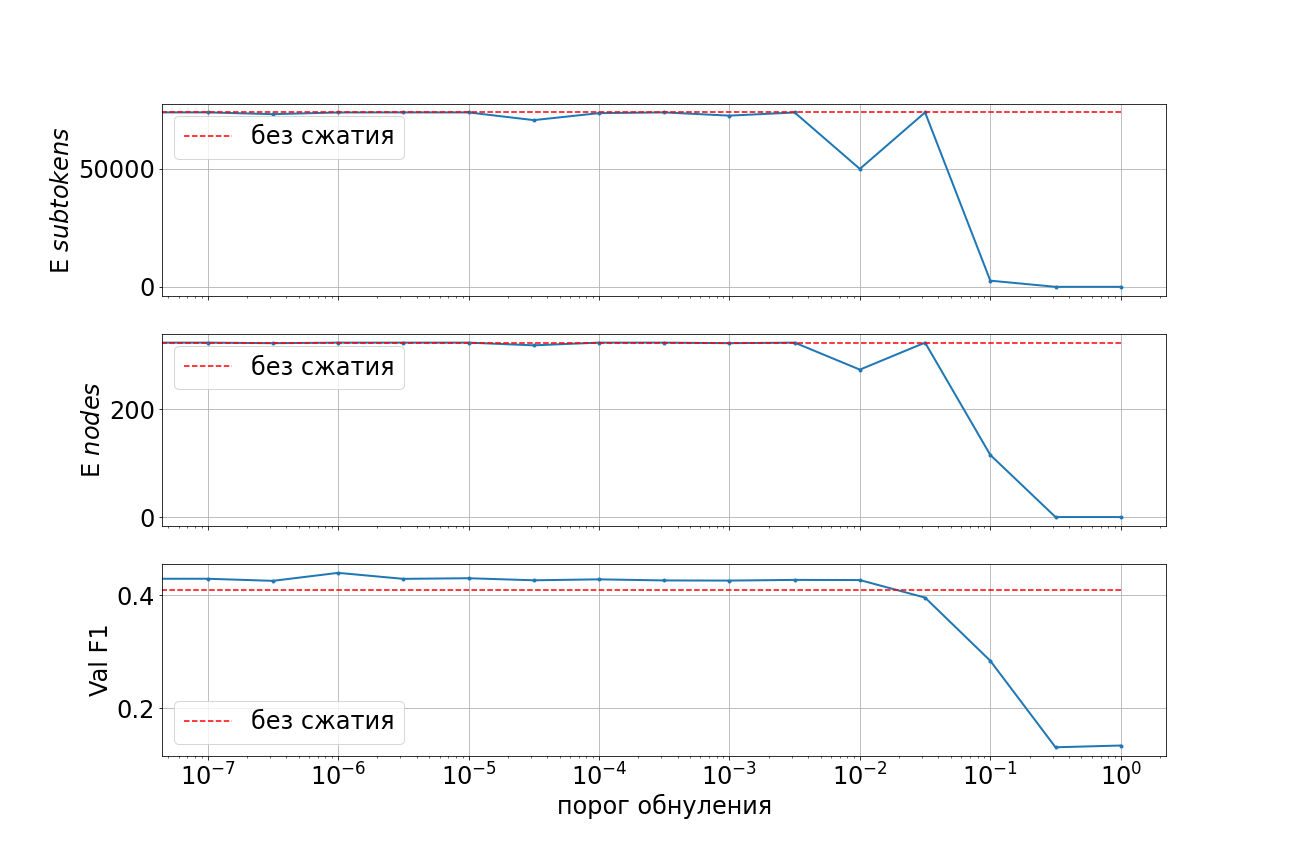
\includegraphics[width=0.8\textwidth]{example.png}
	\caption{Пример графика. Тут должна быть подпись, поясняющая что происходит на рисунке (краткая, но достаточная для понимания основной идеи графика).}
	\label{fig:by_epochs}
\end{figure}

Все рисунки в тексте должны иметь подписи и вы на них должны ссылаться в тексте. Например, на Рисунке~\ref{fig:by_epochs} изображен пример графика. Не забывайте подписывать все оси на графиках, добавлять легенду и пояснять все обозначения, а также используйте адекватного размера шрифты и толщину линий на графиках (все должно быть видно и понятно без многократного увеличения). На рисунке из примера явно не хватает обозначения синей линии в легенде.


\subsection{Таблицы}

Все таблицы в тексте тоже должны иметь подписи и вы на них должны ссылаться в тексте. Например, в Таблице~\ref{table:long_epochs} показаны результаты примерного эксперимента. 


\begin{table}[ht]
	\caption{Пример таблички. Тут должна быть подпись, поясняющая что происходит в таблице (краткая, но по делу).}
	\label{table:long_epochs}
	\footnotesize
	\centering
	\begin{tabular}{lrrrrrrrr}
		\toprule
		& \multicolumn{3}{c}{$\mathsf{Val}$} &
		\multicolumn{3}{c}{$\mathsf{Test}$} \\
		\cmidrule(lr){2-4} \cmidrule(l){5-7} 
		{} &  $\mathsf{Prec}$ &  $\mathsf{Rec}$ &  $\mathsf{F1}$ &  $\mathsf{Prec}$ &  $\mathsf{Rec}$ &  $\mathsf{F1}$  &  $\mathsf{nodes}$ & $\mathsf{subtokens}$\\
		\midrule
		запуск 1    &    0.4894 &   0.3775 &  0.4263 &     0.4824 &    0.3683 &   0.4177 & 10029 & 179\\
		запуск 2    &    0.4887 &   0.3739 &  0.4237 &     0.4891 &    0.3724 &   0.4228 & 10039 & 177\\
		запуск 3    &    0.4820 &   0.3751 &  0.4219 &     0.4838 &    0.3677 &   0.4178 & 10037&	180\\
		\midrule
		\bf{среднее} &    \bf{0.4867} &   \bf{0.3755} &  \bf{0.4239} &    \bf{ 0.4851} &    \bf{0.3695} &   \bf{0.4195} \\
		\bf{дисперсия}  &    0.0041 &   0.0019 &  0.0022 &     0.0036 &    0.0025 &   0.0029 \\
		\bottomrule
	\end{tabular}
\end{table}

\subsection{Формулы}

Формулы стоит центрировать, а также нумеровать, если вы ссылаете на них в тексте. Также не забывайте пояснять все обозначения в формулах. Например, запишем следующую задачу оптимизации:
\begin{equation}
    \label{eq:si_opt}
        \theta* = \min_{\theta} F(\theta),
\end{equation}
где $F$~-- квадратичная функция от параметра $\theta$. При необходимости, далее в тексте можно сослаться на формулу~(\ref{eq:si_opt}). При этом, в зависимости от конкретных формул, можно использовать разные слова: формула, уравнение, задача оптимизации и т.п.

	
\newpage 
\nocite{*}
\printbibliography[heading=bibintoc] 


% \begin{thebibliography}{0}
% 	\bibitem{chirkova18}\hypertarget{chirkova18}{}
% 	\href{https://arxiv.org/abs/1810.10927}
% 	{Nadezhda Chirkova, Ekaterina Lobacheva, Dmitry Vetrov. Bayesian Compression for Natural Language Processing. In EMNLP 2018.}
% \end{thebibliography}
	
\newpage
\appendix

\section{Пример секции аппендикса}
\end{comment}


\newpage
\printbibliography[heading=bibintoc] 







\end{document}
